\section{Theorie}
\label{sec:Theorie}
Brückenschaltungen werden in der Physik verwendet, um über bereits bekannte Bauelemente die
physikalischen Kennwerte eines unbekannten ohmschen Widerstands oder einer Impedanz zu bestimmen.
Mithilfe der beiden Kirchhoffschen Regeln lassen sich Bedingungen zur Bestimmung unbekannter Elemente in
Brückenschaltungen formulieren.
\subsection{Kirchhoff'sche Regel}

\subsubsection{Knotenregel}
Die Knotenregel besagt anschaulich, dass Ströme, die in einen Knotenpunkt
hineinfließen, auch wieder hinausfließen müssen. Im Knoten selbst dürfen also keine Ströme verschwinden,
oder neu entstehen.
\begin{equation}
  \centering
  \label{eqn:knotenregel}
\sum_{k}{I_K}=0
\end{equation}
Etwas mathematischer ausgedrückt heißt das, dass die Summe über alle eingehenden
und alle ausgehenden Strömen gleich Null sein muss.

\subsubsection{Maschenregel}
Eine Masche bezeichnet einen in sich geschlossenen Stromkreis.
Die Maschenregel besagt, dass für eine Masche die Summe aller Einzelspannungen $U_i$
an den einzelnen Bauelementen, wie zum Beispiel Ohmschen Widerständen, Spulen und Kondensatoren,
gleich der angelegten Gesamtspannung $U_0$ sein muss. Äquivalent dazu ist die Formulierung, dass die Summe aller auftretenden Spannungen $U_k$ gleich Null ist.

\begin{equation}
  \label{eqn:maschenregel}
  \centering
U_0=\sum_{i}{U_i} \Rightarrow \sum_{k}{U_k}=0
\end{equation}
 Eine alternative Formulierung erhält man unter Verwendung des Ohmschen Gesetz. Dieses definiert den elektrischen Widerstand $R$
 als Quotienten aus der anliegenden Spannung $U$ zur Stromstärke $I$ des durch den Widerstand fließenden Stroms.
 Stellt man das Ohmsche Gesetz nach $U$ um, ergibt sich der Zusammenhang
\begin{equation}
   \centering
   U=R \cdot I
 \end{equation}
 Somit kann die Maschenregel auch abhängig von Stromstärke und Widerständen formuliert werden:
 \begin{equation}
   U_0=\sum_{i}{I_i \cdot R_i}
\end{equation}


\begin{figure}
  \centering
  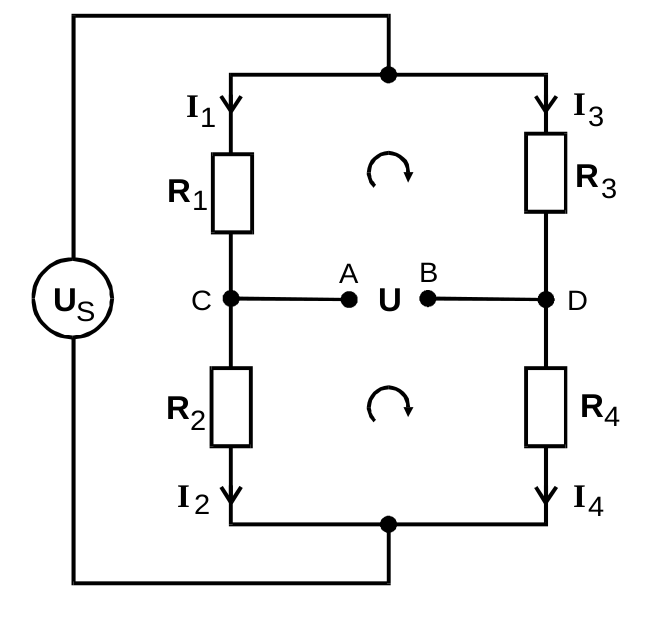
\includegraphics[width=0.9\textwidth]{Bilder/brueckenschaltungallgemein.png}
  \caption{Grundlegender Aufbau einer Brückenschaltung \cite{Anleitung}}
  \label{fig:brückenschaltung}
\end{figure}
In Abbildung \ref{fig:brückenschaltung} ist der schematische Aufbau einer Brückenschaltung dargestellt.
Als Brückenspannung wird hierbei die zwischen den Punkten $A$ und $B$ auftretende Spannung $U_{Br}$ bezeichnet.

Die Brückenschaltung kann man als Parallelschaltung zweier widerstandsbehafteter Leiter verstehen. An diese Parallelschaltung wird dabei die Speisespannung $U_S$ angelegt.
Der Stromfluss teilt sich auf die beiden parallelen Zweige auf. Er fließt damit entweder durch den linken Zweig und somit durch die Widerstände $R_1$ und $R_2$ oder durch den rechten Zweig, also durch $R_3$ und $R_4$.

Mithilfe der Kirchhoffschen Regeln \eqref{eqn:knotenregel} und \eqref{eqn:maschenregel} lässt sich die Brückenspannung $U_{Br}$ abhängig von den verwendeten Widerständen und der angelegten Spannung $U_S$ wie folgt formulieren:
\begin{equation}
  \label{eqn:brückeeingang}
U_{Br}=\frac{R_2R_3-R_1R_4}{(R_3+R_4)(R_1+R_2)}U_S .
\end{equation}
Die Brückenspannung verschwindet, wenn der Zähler gleich Null, also $R_2R_3-R_1R_4=0$ gilt.
Die Brücke wird dann als abgeglichen bezeichnet. Es gilt also:
\begin{equation}
R_2R_3=R_1R_4
\label{eqn:abgleichbedingung}
\end{equation}
Diese sogenannte Abgleichbedingung hängt somit lediglich von den Widerständen ab. Somit lässt sich ein unbekannter Widerstand $R_x$ mittels der abgeglichenen Brücke bestimmen.

Dafür müssen die bekannten Widerstände mit möglichst großer Genauigkeit bekannt sein und mindestens einer der Widerstände muss sich regulieren lassen.

Um eine möglichst genaue Bestimmung des unbekannten Widerstands $R_x$ zu realisieren, muss man die Brückenspannung möglichst genau zu Null abgleichen können.
Dazu wird ein Galvanometer, (Mikro-)Voltmeter oder ein Kathodenstrahloszillograph verwendet.

Da nach Gleichung \eqref{eqn:brückeeingang} ein Zusammenhang zwischen der Speisespannung $U_S$ und der Brückenspannung $U_{Br}$ besteht, wird die Genauigkeit der Messung zudem durch eine möglichst große Speisespannung verbessert.
Schließlich kann anstelle eines ohmschen Widerstands auch ein komplexer Widerstand mittels der abgeglichenen Brücke bestimmt werden. Hierfür muss man allerdings beachten, dass dieser sich aus einen Wirk-und einen Blindwiderstand zusammensetzt.

\subsection{Realisierung komplexer Widerstände von Induktivitäten und Kondensatoren}
\label{sec:komplexewiderstände}
Fließt Strom durch einen Kondensator, so baut sich in diesem ein elektrisches Feld auf. Ähnlich verhält es sich bei Spulen. Hier baut sich bei fließendem Strom ein magnetisches Feld auf.
Einer Spannungsquelle wird also durch angeschlossene Kondensatoren oder Spulen Energie entzogen und im elektrischen bzw. magnetischen Feld gespeichert. Diese wird allerdings nicht umgewandelt in eine andere Energie (z.B. thermische oder mechanische) sondern kann nach einer Umkehrung der Spannungsrichtung zur Quelle zurückgeführt werden.
Daher werden sogenannte Impedanzen (Wechselstromwiderstände) zur Beschreibung von Spulen und Kondensatoren verwendet:
\begin{equation}
\Theta= X+iY
\end{equation}
$X$ ist hierbei der Wirkwiderstand und $Y$ die Reaktanz (Blindwiderstand).
Bei Spulen und Kondensatoren treten zudem Wärmeverluste, zum Beispiel zwischen den Kondensatorplatten
oder in den Drähten auf.

Zur Realisierung solcher sogenannter dielektrischen Verluste
ergänzt man daher das Ersatzschaltbild durch gedachte ohmsche Widerstände $R_x$.
Brückenschaltungen mit komplexen Widerständen müssen somit im Gegensatz zu Schaltungen, welche lediglich ohmsche Widerstände enthalten, mit Wechselstrom betrieben werden, sodass das magnetische bzw. elektrische Feld sich periodisch auf- und auch wieder abbauen kann.

Somit müssen wiederum die Abgleichbedingungen für den Fall, dass Kondensatoren und Spulen in der Brückenschaltung verwendet werden, sowohl Phase, als auch den Wirkwiderstand berücksichtigen.
Im Folgenden soll im Einzelnen auf die fünf verschiedenen Brückenschaltungen eingegangen werden.

\subsection{Wheatstonesche Brückenschaltung}
\begin{figure}
  \centering
  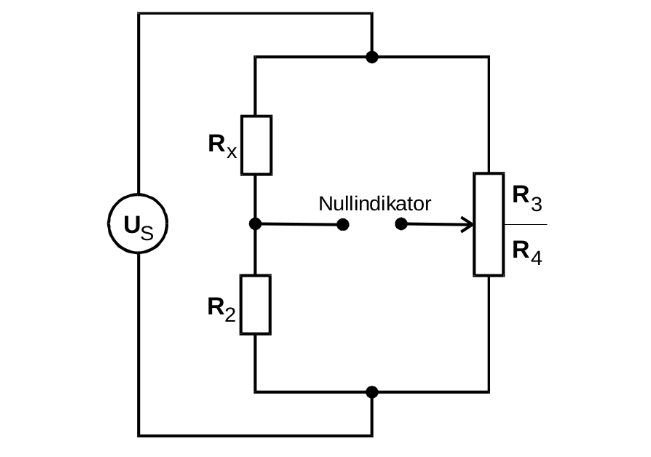
\includegraphics[width=0.9\textwidth]{Bilder/Wheatstone_bruecke.png}
  \caption{Wheatstonesche Brückenschaltung zur Bestimmung eines unbekannten Widerstands \cite{Anleitung}}
  \label{fig:wheatstonebrücke}
\end{figure}

In Schaltbild \ref{fig:wheatstonebrücke} ist die Wheatstonesche Brücke abgebildet. Diese enthält lediglich Ohmsche Widerstände. Daher kann sie sowohl mit Wechselstrom als auch mit Gleichstrom betrieben werden.
Der zu bestimmende Widerstand $R_x$ lässt sich nach \eqref{eqn:abgleichbedingung} über die anderen Widerstände wie folgt bestimmen:
\begin{equation}
  \centering
  R_x=R_2 \cdot \frac{R_3}{R_4};
\label{eqn:widerstand}
\end{equation}
Aus \eqref{eqn:widerstand} ergibt sich, dass die konkreten Werte von $R_3$ und $R_4$ nicht bekannt sein müssen, um $R_x$ zu ermitteln. Es reicht vollkommen, ihr Verhältnis zu kennen.
Daher können $R_3$ und $R_4$ mittels eines Potentiometers realisiert werden.

\subsection{Kapazitätsmessbrücke}
\begin{figure}
  \centering
  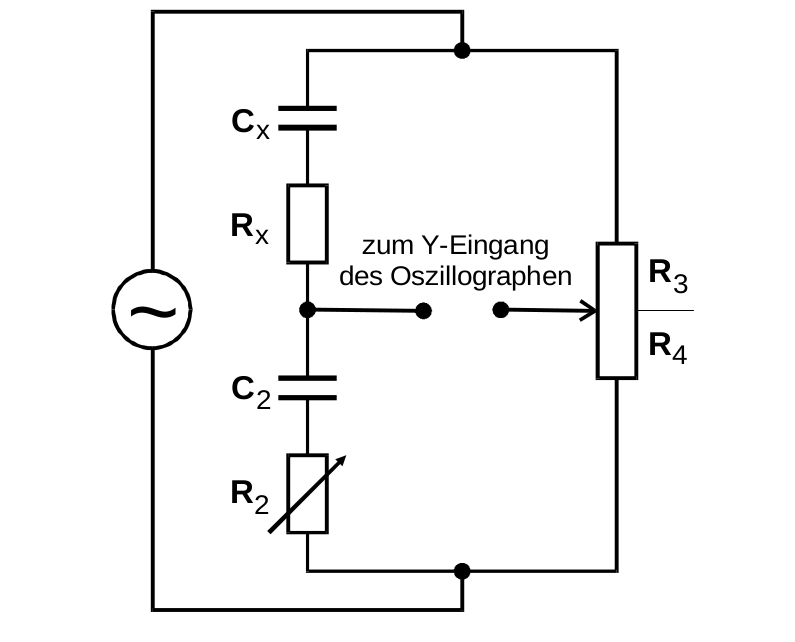
\includegraphics[width=0.7\textwidth]{Bilder/kapazitaetmessbruecke.png}
  \caption{Brückenschaltung zur Bestimmung eines unbekannten Kondensators \cite{Anleitung}}
  \label{fig:kapazitätsmessbrücke}
\end{figure}
Bei der Kapazitätsmessbrücke abgebildet in \ref{fig:kapazitätsmessbrücke} wird ein Kondensator in die Brückenschaltung eingebaut.
Wie bereits in \ref{sec:komplexewiderstände} erklärt, muss daher sowohl die Phase, als auch der Wirkwiderstand abgeglichen werden.
$R_x$ steht hierbei stellvertretend für die Wärmeverluste im Kondensator. Zum Abgleich des komplexen kapazitiven Widerstands wird also eine Ersatzschaltung verwendet.
Hierzu wird ein bekannter Kondensator $C_2$ in Reihe geschaltet zu einem regulierbaren ohmschen Widerstand $R_2$.
$R_2$ ist hierbei regulierbar, um die in der Kapazität entstehende Phasenverschiebung zu kompensieren. Für den $R_2-C_2$-Zweig wird hierbei angenommen, dass $R_{Wirk}=R_2$ gilt, also der Kondensator $C_2$ verlustfrei ist. Dies ist, wie sich auch anhand von $R_x$ nahezu 0 zeigt, realisierbar.
Wenn der unbekannte Kondensator als verlustfrei angenommen werden kann, kann auf den regelbaren Widerstand $R_2$ verzichtet werden.
Dies würde sich auch in der Messung zeigen. Wenn $R_2$ auf $0 \Omega$ gestellt werden kann und sich die Brückenspannnung trotzdem zu Null abgleichen lässt, kann man den Kondensator als verlustfrei annehmen.
Die Abgleichbedingungen ergeben sich somit zu
\begin{equation}
\centering
\label{eqn:kapwiderstand}
R_x=\frac{R_2R_3}{R_4}
\end{equation}
und
\begin{equation}
\centering
\label{eqn:kapazitaet}
C_x=\frac{C_2R_4}{R_3}
\end{equation}
Aus den Abgleichbedingungen ist ersichtlich, dass das Verhältnis von $R_3$ zu $R_4$ mit \eqref{eqn:kapazitaet} unabhängig von $R_x$ formuliert werden kann.
Die Notwendigkeit der zweiten Abgleichbedingung und damit das Hinzufügen eines ohmschen Widerstands $R_2$ ergibt sich somit nur, wenn $R_x$ ungleich 0 ist.

\subsection{Induktivitätsmessbrücke}

\begin{figure}
  \centering
  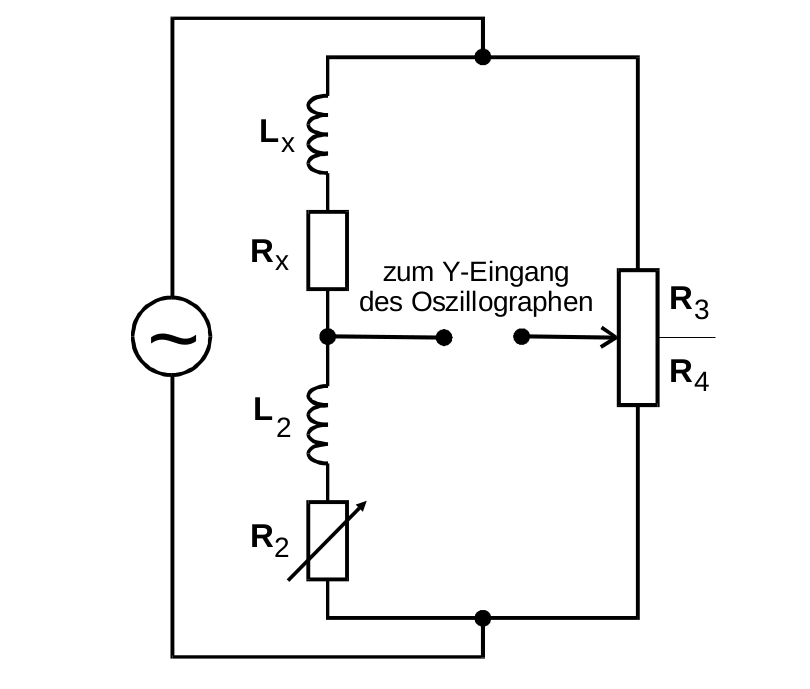
\includegraphics[width=0.9\textwidth]{Bilder/Messbruecke_Spule_mit_R.png}
  \caption{Brückenschaltung zur Bestimmung der Induktivität einer Spule  \cite{Anleitung}}
  \label{fig:induktivitätsmessbrücke}
\end{figure}
In Schaltbild \ref{fig:induktivitätsmessbrücke} ist eine Brückenschaltung zur Messung eines induktiven Widerstands dargestellt.
Es müssen also erneut komplexe Widerstände betrachtet werden. Der prinzipielle Aufbau zur Messung einer realen Spule stellt sich also sehr ähnlich wie die Brückenschaltung zur Bestimmung eines Kondensators dar.
Es müssen lediglich die Kondensatoren $C_i$ an entsprechender Stelle durch Spulen $L_i$ ersetzt werden.
Die Abgleichbedingungen ergeben sich somit zu:
\begin{equation}
\centering
\label{eqn:indukwiderstand}
R_x=\frac{R_2R_3}{R_4}
\end{equation}
und
\begin{equation}
\centering
\label{eqn:induktivität}
L_x=\frac{L_2R_3}{R_4}
\end{equation}
Die bei der Kapazitätsmessbrücke leicht zu realisierende Forderung, dass der Wirkwiderstand im linken unteren Zweigabschnitt gleich dem Widerstand $R_2$ ist,
lässt sich bei Induktivitäten besonders für niedrige Frequenzen nur schwerlich realisieren.
Es lassen sich daher genauere Ergebnisse erzielen, wenn anstelle der Induktivität $L_2$ eine Ersatzschaltung mit einer Kapazität, die sogenannte Maxwell-Brücke, verwendet wird.

\subsection{Maxwell-Brücke}
\begin{figure}
  \centering
  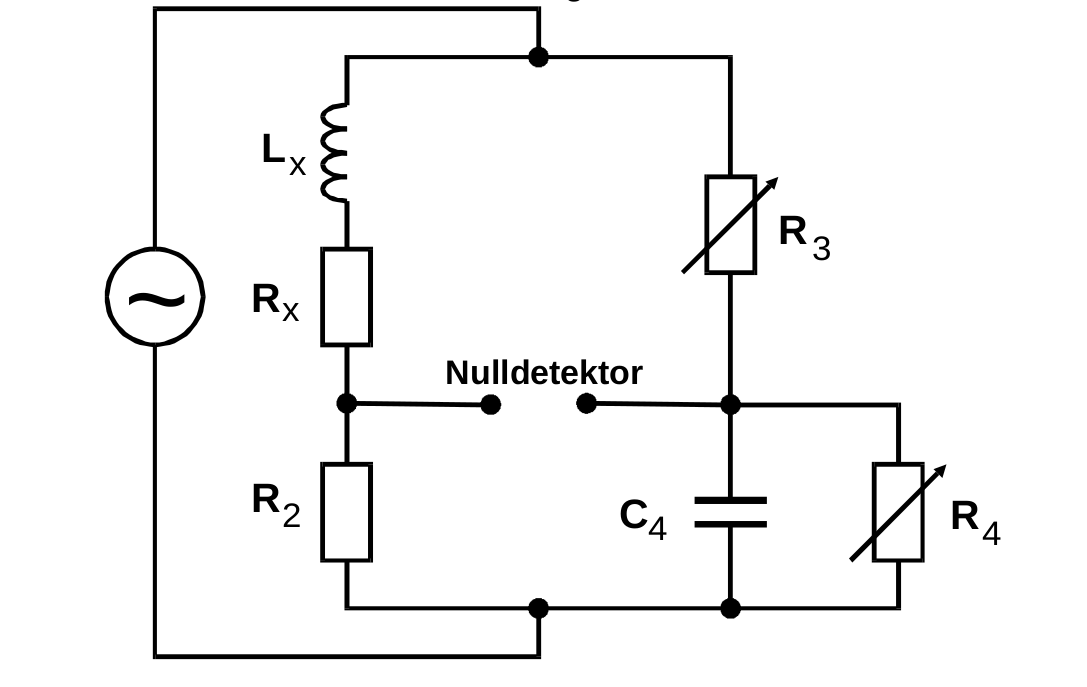
\includegraphics[width=0.9\textwidth]{Bilder/maxwell_bruecke.png}
  \caption{Maxwell-Brücke zur Bestimmung einer Induktivität \cite{Anleitung}}
  \label{fig:maxwellbrücke}
\end{figure}
In der in Abbildung \ref{fig:maxwellbrücke} werden erneut Induktivitäten vermessen.
Wie bereits erwähnt, erzielt man im Gegensatz zur Induktivitätsmessbrücke
mit einer Induktivität $L_2$ hier mit einer eingebauten Kapazität $C_2$ aufgrund der deutlich geringeren Wärmeverluste eine höhere Genauigkeit der messung.
Für die Abgleichbedingungen erhält man, indem man erneut die Kirchhoffschen Regeln nach \eqref{eqn:maschenregel} und \eqref{eqn:knotenregel} verwendet, zu:
\begin{equation}
\centering
R_x=\frac{R_2R_3}{R_4}
\end{equation}
und
\begin{equation}
\centering
\label{eqn:maxwellinduktivität}
L_x=R_2R_3C_4
\end{equation}
\subsection{Wien-Robinson-Brücke}
\begin{figure}
  \centering
  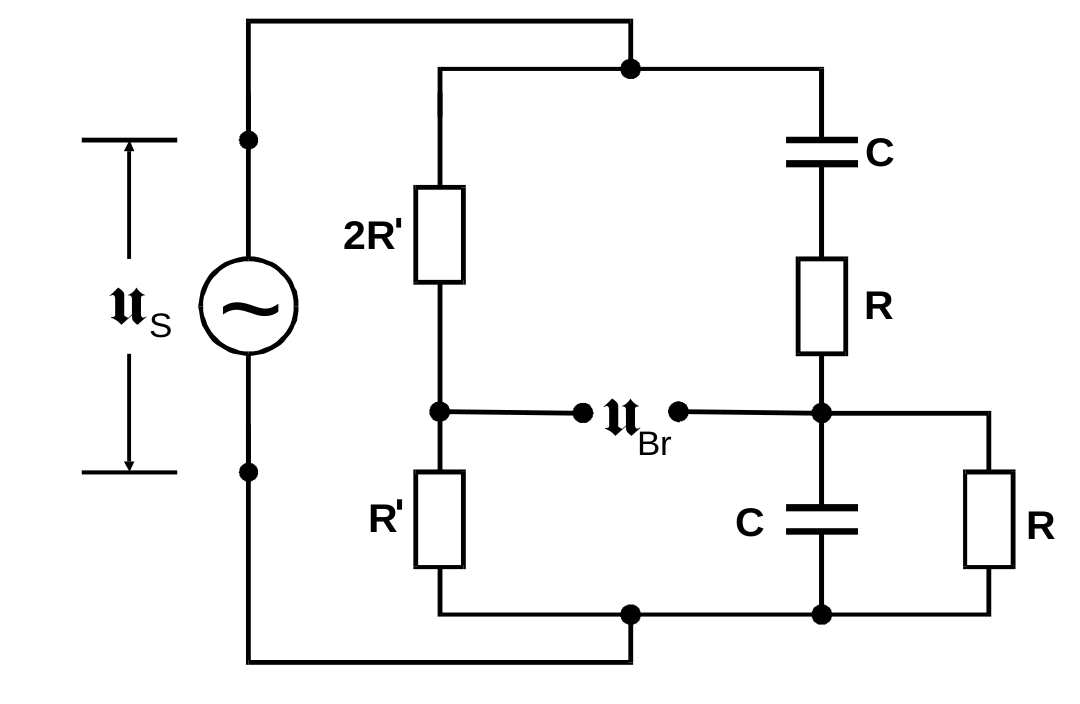
\includegraphics[width=0.9\textwidth]{Bilder/wien_robinson_bruecke.png}
  \caption{Wien-Robinson-Brücke zur Klirrfaktor-Bestimmung \cite{Anleitung}}
  \label{fig:wienrobinsonbrücke}
\end{figure}

In der letzten betrachteten Brückenschaltung sind im Gegensatz zu den vorherigen Brückenschaltungen keine Abgleichelemente enthalten.
Bei den zuvor betrachteten Brückenschaltungen sollte sich prinzipiell also die Abgleichbedingung immer unabhängig von der Frequenz $\omega$ der Speisespannung $U_S$ erfüllen lassen. Dies stimmt allerdings nur eingeschränkt. Für große Frequenzen $\omega$ werden sich allerdings störende Streueffekte zeigen und für kleine Frequenzen dauert es etwas, bis sich ein stationärer Fall einstellt.

Die Wien-Robinson-Brücke dient nun als elektronischer Filter, das heißt, im Gegensatz zu den bisherigen Schaltungen wird die Wien-Robinson-Brücke sich nur bei einer bestimmten Frequenz $\omega=\omega_0$ abgleichen lassen.

Die Ableichbedingung ergibt sich somit über die Frequenz.

Der Quotient aus Speise-und Brückenspannung ergibt sich unter der Verwendung komplexer Widerstände und Kapazitäten zu:

\begin{equation}
\label{eqn:wienquotient}
\left|\frac{U_{Br}}{U_s}\right|^2= \frac{(\omega^2R^2C^2-1)^2}{9 \cdot ((1-\omega^2R^2C^2)^2+9\omega^2R^2C^2)}
\end{equation}

Es ist sofort ersichtlich, dass der Zähler=0 ist, die Brückenspannung also verschwindet für
\begin{equation}
  \label{eqn:Omega}
\omega=\omega_0=\frac{1}{RC} .
\end{equation}
Somit lässt sich \eqref{eqn:wienquotient} vereinfacht darstellen durch die Einführung des Frequenzverhältnis:
\begin{equation}
\Omega:=\frac{\omega}{\omega_0}
\end{equation}
Der Quotient der Spannungen wird damit zu

\begin{equation}
\label{eqn:wienquotienteinfach}
\left|\frac{U_{Br}}{U_s}\right|^2= \frac{1}{9}\frac{(\Omega-1)^2}{(1-\Omega^2)^2+9\Omega^2}
\end{equation}
Die Filterfunktion der Wien-Robinson-Brücke schlägt somit bei $\omega_0$ nach \eqref{eqn:Omega} zu. Das heißt, dass $\omega_0$ aus dem kontinuierlichen Frequenzspektrum herausgefiltert wird und die umgebenden Frequenzen stark abgeschwächt werden.
\subsubsection{Klirrfaktor-Messung}

In einer idealen Wien-Robinson-Brücke unter Verwendung eines idealen Sinusspannungsgerenators würde die Brückenpannung bei der Frequenz $\omega_0$ verschwinden. Im realen Fall wird allerdings trotzdem eine von Null verschiedene Spannung $U_{Br}$ festgestellt.
Diese entsteht durch Oberwellen, welche ungewollt durch den Sinusgenerator erzeugt werden. Im idealen Fall enthält eine Sinusschwingung keine Oberwellen. Um eine Aussage über die Güte des realen Sinusgenerators zu erhalten, wird der sogenannte Klirrfaktor bestimmt.
Der Klirrfaktor setzt hierbei die Oberwellen ins Verhältnis zur Grundwelle. Ein kleiner Klirrfaktor kennzeichnet somit einen guten Sinusgenerator.
Allgemein berechnet sich der Klirrfaktor zu
\begin{equation}
k:=\frac{\sqrt{\sum_{i=2}^{N}{U_i^2}}}{U_1}
\end{equation}
Im vorliegenden Fall wird vereinfachend lediglich die zweite Oberwelle berücksichtigt.
\begin{equation}
  \label{eqn:klirrfaktor}
k:=\frac{U_2}{U_1}
\end{equation}
